\documentclass[11pt,oneside]{report}
\usepackage[utf8]{inputenc}
\usepackage{graphicx}
\usepackage[german]{babel}
\usepackage{blindtext}
\usepackage{graphicx}
\graphicspath{ {./images/} }
\usepackage{geometry}
 \geometry{
 a4paper,
 left=30mm,
 right=15mm,
 top=20mm,
 bottom=40mm,
 }
\usepackage{helvet}
\renewcommand{\familydefault}{\sfdefault}
\renewcommand{\baselinestretch}{1.5}


\begin{document}

\begin{titlepage}
    \begin{center}
        \vspace*{1cm}
            
        \Huge
        \textbf{Maschinelles Lernen}
            
        \vspace{0.5cm}
        \LARGE
        als Projektarbeit im Informatikunterricht
            
        \vspace{1.5cm}
            
        \textbf{Jonas Groß-Hartmann}
            
        \vfill
        
        \Large
        Fach: Informatik\\
        Fachlehrer: Herr Boettcher\\
        Datum: 11.03.2024
            
    \end{center}
\end{titlepage}


\setcounter{page}{2}
\tableofcontents

\newpage


\section{Einführung}
\blindtext


\chapter{Theoretische Grundlagen}

\section{Maschinelles Lernen}
Maschinelles Lernen ist eines der wichtigsten Teilgebiete der Künstlichen Intelligenz.\footnote{Schmid, Ute (2022): Maschinelles Lernen, URL: https://www.bidt.digital/glossar/maschinelles-lernen/, Stand: 29.01.2024} Unter Maschinellem Lernen (englisch: Machine Learning) versteht man einen Vorgang, bei dem ein System automatisch Muster und Zusammenhänge aus Daten erkennt und sich mit der Zeit verbessert, ohne dabei explizit programmiert worden zu sein. Daher wird Maschinelles Lernen häufig in Wirtschaft, Forschung und Entwicklung verwendet. Man kann dabei Werte vorhersagen, Wahrscheinlichkeiten berechnen, Gruppen und Zusammenhänge in Daten erkennen, Dimensionen ohne großen Informationsverlust reduzieren und Geschäftsprozesse optimieren.\footnote{vgl. Wuttke, Laurenz (2023): Machine Learning: Definition, Algorithmen, Methoden und Beispiele, URL: https://datasolut.com/was-ist-machine-learning/ , Stand: 29.01.2024}

\subsection{Funktionsweise}
Bei Maschinellem Lernen wird einem Modell Informationen gegeben. Dieses Programm erkennt nun Zusammenhänge und Muster zwischen den Eingabewerten und gibt daraufhin einen Wert aus. Dafür wird dem Modell zunächst als Training ein Datenset übermittelt, mit dem es trainiert wird. Dabei überprüft sich das Modell selbst, da mit den Daten auch die gewünschte Zielvariable übermittelt wird. Nachdem das Modell trainiert wurde werden ihm neue, unbekannte Daten übermittelt mit deren Hilfe das Modell nun Vorhersagen treffen kann. Es findet also keine Programmierung im klassischen Sinne statt, da das Programm sich selbst trainiert und programmiert.\footnote{ebd.}

\subsection{Arten des Machine Learnings}
Es gibt vier verschiedene Arten von Maschinellem Lernen, welche verschieden Strategien verwenden und daher verschiedene Anwendungsbereiche abdecken.

%\subsubsection{Überwachtes Lernen}
Das überwachte Lernen (eng.: Supervised Learning) verwendet bekannte Daten, um aus diesen zu lernen. Der Algorithmus erkennt dabei einen Zusammenhang zwischen den Eingabedaten und der Zielvariable. Dies wird zum Beispiel zur Klassifikation und zur Vorhersage von Daten verwendet.

%\subsubsection{Unüberwachtes Lerne}
Das unüberwachte Lernen (eng.: Unsupervised Learning) dagegen hat keine vorgegebenen Zielvariable. Das Modell erkennt hier selbstständig zusammenhänge zwischen den Eingabedaten und gibt diese als Gruppen aus. Daher wird dies zur Clusteranalyse („Eine Clusteranalyse ist ein exploratives Verfahren, um Datensätze hinsichtlich ihrer Ähnlichkeit in Gruppen einzuteilen“\footnote{Wuttke, Laurenz (2022): Clusteranalyse einfach erklärt, URL:https://datasolut.com/wiki/clusteranalyse/, Stand: 02.03.2024}) und zur Dimensionsreduktion verwendet.

%\subsubsection{Teilüberwachtes Lernen}
Das teilüberwachte Lernen (eng.: Semi-Supervised Learning) ist eine Mischung aus über- wachtem und unüberwachtem Lernen, da hier eine geringe Menge an Daten mit Zielvariable und eine große Menge ohne Zielvariable genutzt werden. Dadurch werden weniger bekannte Daten benötigt, was häufig kostengünstiger und weniger Arbeitsintensiv ist, da Daten meist manuell einer Zielvariable zugewiesen werden müssen.

%\subsubsection{Verstärkendes Lernen}
Das verstärkende Lernen (eng.: Reinforcement Learning) verfolgt eine andere Idee des Machine Learnings. Das Programm hat keinen Trainingsdatensatz, es belohnt und bestraft sich durch verschiedene Handlungen mithilfe einer Kostenfunktion. Der Algorithmus weiß also nicht, was die richtige Handlung ist. Er versucht, ein Ziel zu erreichen und dabei die Kosten, welche durch die Kostenfunktion bestimmt werden, möglichst klein zu halten.

Da in dieser Arbeit ein Programm zur Bilderklassifizierung erstellt wird, wird ein Modell mit überwachtem Lernne verwendet. Dies wird meistens zur Klassifizierung von Daten, wie beispielsweise Bildern, verwendet. Daher wird auch ein Datensatz mit beschrifteten Bildern benötigt.\footnote{vgl. Wuttke(2023)}


\section{Neuronale Netzwerke}
Ein Grundbestandteil des Machine Learnings und von KI generell ist das künstliche neuronale Netz. Mit diesem kann ein Modell aus Daten entscheiden, was der jeweilige Output ist. Ein künstliches neuronales Netz ist einem Nervensystem nachempfunden. Daher hat es einen sehr ähnlichen Aufbau.

\subsection{Neuronen}
Ein Netz besteht aus mehreren Neuronen. Diese haben meist mehrere Inputs und einen Output. Im menschlichen Körper heißen die Inputs Dendriten und der Output Axon und funktionieren wie ein künstliches Neuron. Die Inputs erhält das Neuron dabei meist von anderen Neuronen und gibt Outputs an andere Neuronen weiter. Dadurch entsteht ein Netz aus vielen, zusammenhängenden Neuronen.

\subsection{Aufbau eines Neuronalen Netzes}
Ein Neuronales Netz besteht aus mehreren Schichten, sogenannte „Layer“. Diese Layer bestehen aus beliebig vielen Neuronen, welche mit den Neuronen des vorherigen und des folgenden Layers verbunden sind. Dabei gibt es drei Arten von Layern. Der Input-Layer nimmt die Daten auf, die als Input übergeben werden und ist immer der erste Layer eines künstlichen Neuronalem Netz. Dementsprechent gibt es auch einen Output-Layer, welcher eine Zielvariable ausgibt. In diesem Layer gibt es immer so viele Neuronen, wie es mögliche Outputs gibt. Alle anderen Layer werden als Hidden Layers bezeichnet. Diese sind für die Verarbeitung der Daten verantwortlich. Es kann beliebig viele Hidden Layers geben und diese können beliebig viele Neuronen beinhalten. Außerdem benötigt jeder Layer eine Aktivierungsfunktion, welche bestimmt, ob ein Neuron aktiviert wird.\footnote{Welsch, Stefan (2023): Die Grundlagen neuronaler Netze - Einfach erklärt, URL: https://b-nova.com/home/content/the-basics-of-neural-networks-easily-explained/, Stand: 29.01.2024} Eine Funktion, die häufig dafür verwendet wird, ist die ReLu-Funktion (rectified linear activation function). Sie ist zur Standardaktivierungsfunktion für viele Arten von neuronalen Netzen geworden, da ein Modell, das sie verwendet, leichter zu trainieren ist und oft eine bessere Leistung erzielt.\footnote{vgl. Brownlee, Jason (2020): A Gentle Introduction to the Rectified Linear Unit (ReLU), URL: https://machinelearningmastery.com/rectified-linear-activation-function-for-deep-learning-neural-networks/, Stand: 03.03.2024}


\chapter{Technische Grundlagen}

\section{TensorFlow}
Um ein Machine Learning Modell zu entwickeln kann man verschiedene Bibliotheken und Frameworks verwenden. Ich habe mich für das Framework TensorFlow in Python entschieden, welches für das erstellen von Maschine Learning Modellen gut geeignet ist. Auf der offiziellen Website von TensorFlow sieht man, dass die Bibliothek von vielen großen Firmen genutzt wird wie beispielsweise Google, Coca-Cola und Intel.\footnote{vgl. https://www.tensorflow.org/about/case-studies, Stand: 02.03.2024}

Die Bibliothek kann mithilfe des Befehls \verb+import tensorflow as tf+ importiert werden. „\verb+as tf+“ muss dabei nicht verwendet werden, verkürzt allerdings das Aufrufen der Funktionen und wird in den meisten TensorFlow-Projekten verwendet.

\section{Keras}
Um nun ein Modell erstellen zu können wird die Keras-Bibliothek genutzt. Diese ist Teil von TensorFlow und ist eine relative Einsteigerfreundliche und einfache Software.

Mit Keras kann man ein Sequential Modell erstellen, welches der einfachste Typ eines Modells von Keras ist. Man erstellt dieses mit \verb+model = keras.Sequential()+. Als Parameter kann man nun einen Array angeben, welcher die Layers des neuronalen Netzes enthält. So kann man beispielsweise einen dense-Layer(\verb+layers.Dense(units=64, activation='relu')+) angeben. In dem Beispiel besteht der Layer aus 64 Neuronen und die Aktivierungsfunktion ist eine RuLu-Funktion.

Das Modell muss anschließend kompiliert werden. Die Methode \verb+model.compile()+ kann dafür benutzt werden. Man muss zudem einen Optimizer und eine Verlustfunktion angeben, mit denen das Modell lernt. Um die Genauigkeit des Modells anzeigen zu lassen kann man als metric-Parameter \verb+"accuracy"+ angeben, was Sinnvoll für die Bewertung des Modells ist.

Um das Modell nun zu trainieren wird die \verb+model.fit()+-Methode genutzt. Die Methode benötigt ein Trainings-Datensatz und ein Validation-Datensatz. Das Modell wird mit dem Trainings-Datensatz trainiert, während das Validation-Datensatz zum überprüfen des Datensatzes mit unbekannten Daten verwendet wird. Zudem muss die Anzahl der Epochen übergeben werden, die angibt, wie häufig das Modell trainiert werden soll.

Das Modell kann nun neue Daten vorhersagen mithilfe der \verb+model.predict()+-Methode. Diese benötigt als übergebenen Parameter einen oder mehrere Werte, mithilfe derer das Modell einen neuen Wert vorhersagen kann.\footnote{vgl. https://keras.io/about/, Stand: 03.03.2024}

\section{TensorFlow Lite}
Mithilfe von TensorFlow Lite kann ein fertig trainiertes Modell in einer Datei gespeichert werden, sodass sie zu einem späteren Zeitpunkt wieder aufgerufen und zur Vorhersage von Daten verwendet werden kann. Das Keras-Modell kann dadurch mithilfe folgender Methode zu einem TensorFlow Lite-Modell konvertiert werden: \verb+tf.lite.TFLiteConverter.from_keras_model(model)+. Anschleißend muss dieser Konvertiere mithilfe der Methode \verb+convert()+ das TensorrFlow Lite-Modell konvertieren. Dieses kann nun mit Standard-Pythonfunktionen gespeichert werden (\verb+with open(+ \verb+"model.tflite", 'wb') as f: f.write(tflite_model)+).

Das gespeicherte Modell kann nun jederzeit wieder aufgerufen werden, um Vorhersagen zu tätigen. Dabei muss allerdings beachtet werden, dass die Keras-Funktionen nicht mehr verwendet werden können, da es sich nun um ein TensorFlow Lite-Modell handelt. So kann nicht mehr die \verb+model.predict()+-Methode verwendet werden, da diese Teil eines Kears-Modells ist. Die entpechende Methode für das TensorFlow Lite-Modell ist \verb+classify_lite()['outputs']+. Die Methode benötigt einen Parameter, welcher der Name des Input-Layers ist, also zum Beispiel \verb+classify_lite+ \verb+(sequential_1_input=input)['outputs']+. Der Name des Input-Layers ist hier \verb+sequential_1+ und als Input wird eine Variable \verb+input+ übergeben.\footnote{vgl. https://www.tensorflow.org/tutorials/images/classification,Stand: 03.03.2024}


\chapter{Projekt}

\section{Auswählen des Datensatzes}
Um ein Modell zur Klassifizierung von Bilder erstellen zu können muss zunächst ein Datensatz ausgewählt werden. Dafür habe ich mich für einen Datensatz mit Bildern von Artikeln aus dem Supermarkt entschieden.\footnote{https://github.com/marcusklasson/GroceryStoreDataset, Stand: 10.02.2024} Der Datensatz wurde für eine andere Arbeit erstellt und steht auf der Website GitHub zu Verfügung.\footnote{Klasson, Marcus et al. (2019): A Hierarchical Grocery Store Image Dataset with Visual and Semantic Labels, URL: https://arxiv.org/abs/1901.00711, Stand: 03.03.2024} Der Datensatz wurde von mir in einen einzige Sammlung von Bildern reduziert und in der Programmierung automatisch aufgeteilt, sodass zufällig Bilder für die Modelle in Trainings- und Validationsdatensatz aufgeteilt werden.

\section{Implementierung}
\blindtext

\section{Overfitting}
\blindtext

\section{Ausblick}
\blindtext


\chapter{Fazit}
\blindtext


\appendix
\chapter{Anhang}

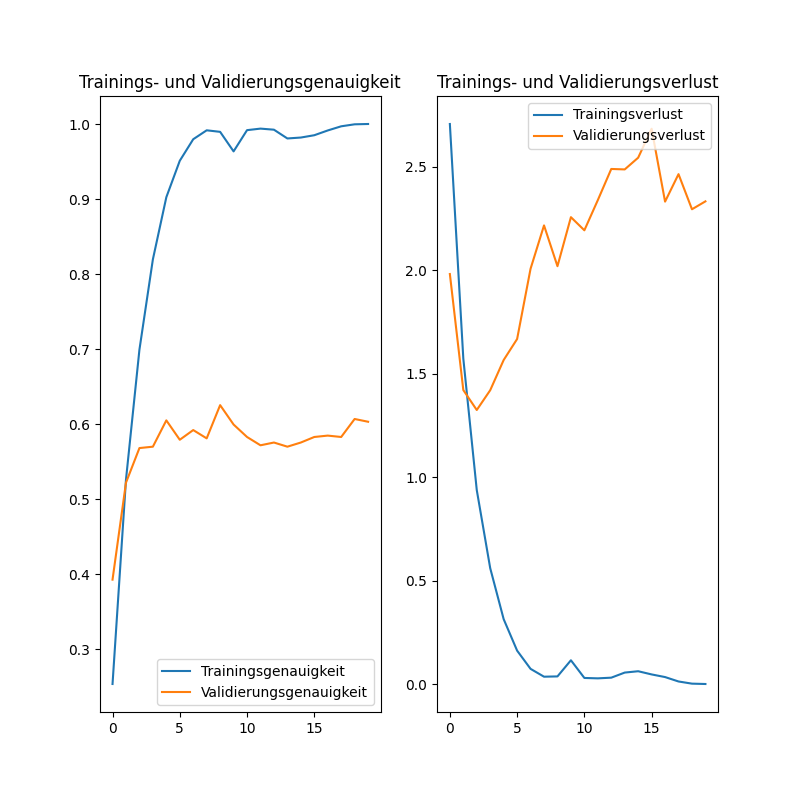
\includegraphics[width=0.7\textwidth]{model_overfitting}

Abb.1: Ergebnisse des ersten Modells mit Overfitting

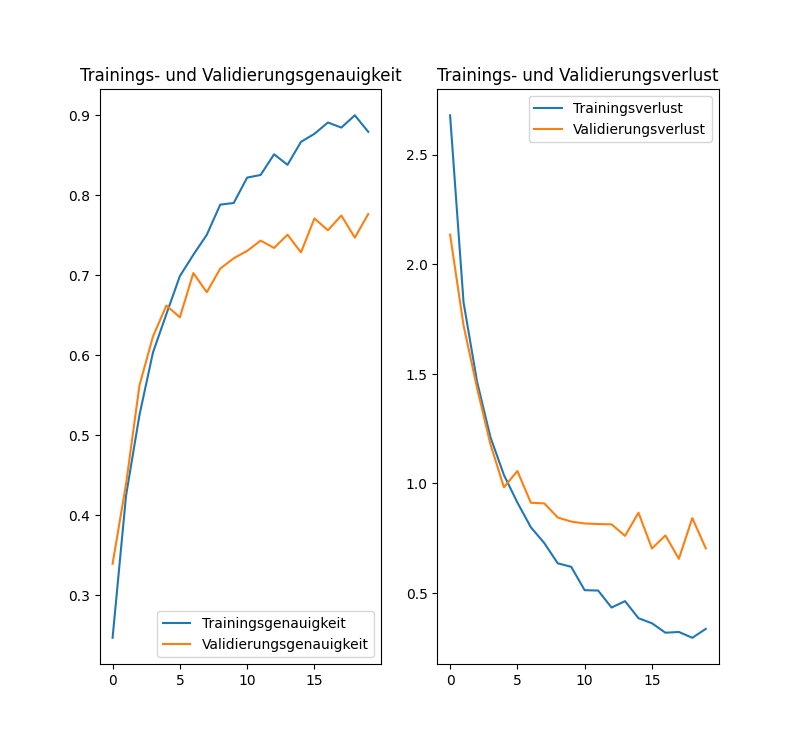
\includegraphics[width=0.7\textwidth]{model}

Abb.2: Ergebnisse des zweiten Modells mit Datenerweiterung und Dropout

\newpage

\includegraphics[width=0.9\textwidth]{selbststaendigkeitserklaerung}


\end{document}